\documentclass[12pt]{book}
\usepackage[utf8]{inputenc}
\usepackage[spanish, mexico]{babel}
\usepackage[table]{xcolor}
\usepackage{graphicx}
\usepackage[export]{adjustbox}
\usepackage{amsmath}
\usepackage{natbib}
\usepackage{amsthm}
\usepackage{amsfonts}
\usepackage{subcaption}
\usepackage{array}
\usepackage{setspace} %setstrech
\usepackage{breqn} %equation break
%\usepackage{algorithmic}
\usepackage[linesnumbered,ruled,spanish,vlined]{algorithm2e}
\usepackage{tikz}
\usepackage{tabularx,ragged2e}
\newcolumntype{C}{>{\Centering\arraybackslash}X} % centered "X" column
\PassOptionsToPackage{hyphens}{url}
\usepackage{url}
\usepackage{hyperref}
\renewcommand{\UrlFont}{\ttfamily\small}
\usetikzlibrary{arrows.meta,
                calc, chains,
                positioning,
                shapes.multipart}
 
\usepackage{algpseudocode}
\usepackage{makecell}
\usepackage{multirow}
\usepackage{booktabs}


\graphicspath{ {images/} }
\theoremstyle{definition}
\newtheorem{definition}{Definición}
\newtheorem{theorem}{Teorema}[section]
\newtheorem{corollary}{Corolario}[theorem]
\newtheorem{lemma}[theorem]{Lema}
\algnewcommand\algorithmicforeach{\textbf{for each}}
\algdef{S}[FOR]{ForEach}[1]{\algorithmicforeach\ #1\ \algorithmicdo}

% \title{
% {Thesis Title}\\
% {\large Centro de Investigación y Estudios Avanzados del IPN}
% }
% \author{David Gustavo Merinos Sosa}
% \date{Day Month Year}
\newenvironment{dedication}
  {
   \thispagestyle{empty}% no header and footer
   \vspace*{\stretch{1}}% some space at the top
   \itshape             % the text is in italics
   \raggedleft          % flush to the right margin
  }
  {\par % end the paragraph
   \vspace{\stretch{3}} % space at bottom is three times that at the top
   \clearpage           % finish off the page
  }
\begin{document}
\thispagestyle{empty}

\begin{tabular}{cc}
\multirow{5}{*}{
\includegraphics[scale=0.5]{cinvestav.png}} & \textsc{Centro de Investigaci\'on y de Estudios Avanzados} \\
  & \textsc{del Instituto Polit\'ecnico Nacional} \\
  & \\
  & \textsc{Unidad Zacatenco} \\
  & \textsc{Departamento de Computaci\'on} \\
\end{tabular}

\vspace{2cm}

\begin{center}
{\setstretch{1.5}
  \textbf{\Large Descomposición de gráficas geométricas completas en thrackles. Un
  enfoque computacional para conjuntos de hasta diez puntos.}\\

  {\large
    \vspace{2cm}
    \begin{small} TESIS QUE PRESENTA \end{small} \\
    \textbf{David Gustavo Merinos Sosa} \\

    \vspace{1cm}
    \begin{small} PARA OBTENER EL GRADO DE \end{small} \\
    \textbf{Maestro en Ciencias en Computaci\'on} \\

    \vspace{2cm}
    \begin{small} DIRECTORA DE LA TESIS \end{small}\\
    \textbf{Dra. María Dolores Lara Cuevas} \\
  }
}
\end{center}

\vfill

\textbf{M\'exico, Ciudad de M\'exico \hfill  2019}
\newpage

% \maketitle
\chapter*{Abstract}
Combinatorial geometry is the area of discrete mathematics and computer science which studies combinatoric properties of geometrical objects with discrete features (such as points, planes, lines or geometric graphs). It is envolved in coloring, symmetry, partition and decomposition problems of said geometrical objects. In this thesis we work on a combinatorial geometry problem, particularly with geometric graphs from which we wish to study a parameter currently known as geometric anti-thickness. We say a drawing or a geometric graph is a set of points in the plane and a set of straight lines connecting pairs of points, called edges. A thrackle is a subset of said edges and its corresponding extreme points such that each pair of edges in the subset either crosses or share an extreme point, a thrackle is maximum when it has the maximum number of edges. Given a graph, if we found the minimal number of thrackles, for every drawing of the graph, such that every edge belongs to exactly one thrackle, we would've found the geometric anti-thickness of the given graph.
Finding the geometric anti-thickness is an open problem in combinatorial geometry. Currently, some lower and upper bounds are known. The lower bound is based on counting how many thrackles in a set are necessary such that the previous conditions hold. The upper bound was obtained by finding a set of thrackles with the previously mentioned conditions of a drawing of the complete graph when its points are in convex position. Note that in the lower bound it is assumed that every pair of maximal thrackles do not share an edge, this is not true for convex position. In the case of the upper bound, the result was achieved by using only one  (convex) drawing and this does not give insight about geometric anti-thickness when the drawing is in non-convex general position. In this thesis we find the exact geometric anti-thickness for complete graphs with up to ten vertices We use algorithms to find thrackles in complete graph drawings, we observed that every pair of maximal thrackles share at least one edge. This allowed us to proove that the lower bound is not tight for graphs with up to ten vertices. Besides, we made observations respecting other geometric properties of thrackles and complete graphs to find a relation between these and geometric anti-thickness.

\chapter*{Resumen}
En el campo de la geometría combinatoria y computacional una gráfica está definida por un conjunto
de vértices $V$ y un conjunto de aristas $E$ de pares de elementos de $V$. Cuando la gráfica tiene
todas las aristas entre pares de vértices decimos que la gráfica es completa. Una gráfica geométrica
es un dibujo de una gráfica en el plano en la que cada vértice es representado por un punto en el
plano y cada arista es representada por un segmento de recta que une dos puntos. Un thrackle
geométrico es una gráfica geométrica en la que cada par de aristas es adyacente o se cruza. El
anti-thickness geométrico de una gráfica es el mínimo número de thrackles que existen en una
descomposición de algún dibujo de la gráfica. Encontrar el anti-thickness de gráficas completas es
un problema abierto y equivale a encontrar el número cromático de una gráfica por lo que es un
problema $NP$-difícil. Actualmente se conoce la cota inferior y la cota superior del anti-thickness
geométrico para gráficas completas. La cota inferior se basa en contar cuántos thrackles son
necesarios en una descomposición de tal manera que la unión de sus aristas sea el conjunto de las
aristas de la gráfica completa y la cota superior se basa en encontrar una descomposición en
thrackles de un dibujo de la gráfica completa cuando sus puntos están en posición convexa. En esta
tesis encontramos el anti-thickness geométrico exacto para gráficas completas con hasta diez
vértices. Usamos algoritmos computacionales para buscar thrackles en dibujos de gráficas completas
y observamos que cada par de thrackles máximos se intersecta en al menos una arista lo que nos
permitió probar que la cota inferior no es justa para gráficas con hasta diez vértices. Además
hicimos observaciones con respecto a otras propiedades geométricas de los thrackles y las
gráficas completas como el número de cruce y la reflexividad de un conjunto de puntos.

\chapter*{Dedicación}
\begin{dedication}
A mi hermano Eduardo, a mis padres María e Isaías, a Jehová mi Dios. 
\end{dedication}

\chapter*{Agradecimientos}
Agradezco al CONACYT sin el cual no habría sido posible completar este programa de 
maestría. Estoy también muy agradecido con mi asesora de tesis, la Doctora María Dolores
Lara Cuevas por aceptarme como tesista y apoyarme en todo momento en el desarrollo de
este trabajo. Gracias a mis compañeros de generación por las incontables horas de
diversión.

\tableofcontents

\chapter{Introducción}
Un dibujo rectilíneo de una gráfica, también llamado gráfica geométrica, está definido por un conjunto de
puntos en el plano, llamados vértices, y un conjunto de segmentos de recta que unen pares de puntos,
llamados aristas. Un thrackle es un subconjunto de estos segmentos tal que cada par se cruza o tiene un
extremo en común. En el área de geometría combinatoria existe un problema en el que, dada una gráfica, se
busca saber cuál es el mínimo número de thrackles que existen en un conjunto de tal manera que cada
thrackle tiene una de las aristas de un dibujo rectilíneo de la gráfica y no hay dos thrackles del conjunto
que compartan una o más aristas y además, la unión de los thrackles es el conjunto de aristas de la
gráfica. Este parámetro recibe el nombre de anti-thickness geométrico de una gráfica.

El anti-thickness geométrico ha sido estudiado con anterioridad, para gráficas geométricas completas cuyos
vértices están en posición convexa, en el trabajo de \cite{Fabila-Monroy2018}. Denotamos este parámetro
como $At_g(K_n)$; se sabe que \[At_c(K_n) = n - \left\lfloor\sqrt{2n + \frac{1}{4}}-
\frac{1}{2}\right\rfloor.\]

Además, en el trabajo de \cite{Lomeli2018} encuentran el anti-thickness geométrico de una configuración de
puntos conocida como la doble cadena convexa, denotada como $K_{k,l}$. En este trabajo los autores
demuestran que el anti-thickness, $At_g(K_{k,l})$ de la doble cadena convexa es \[ At_g(K_{k,l}) = k+l
-\left\lfloor\sqrt{2l + \frac{1}{4}} -\frac{1}{2}\right\rfloor. \]

En el trabajo de \cite{Dujmovic2017} se ofrecen varios resultados para distintos dibujos de una gráfica, y
además las cotas del anti-thickness geométrico para el caso en el que los puntos de la gráfica completa
están en posición general. Estas cotas son las siguientes:
\[ \frac{n-1}{2} \leq At_g(K_n) \leq n - \left\lfloor\sqrt{2n + \frac{1}{4}}- \frac{1}{2}\right\rfloor.\]

La cota superior proviene de resultado obtenido para el anti-thickness geométrico cuando los puntos están
en posición convexa mientras que la cota inferior proviene del hecho de que un thrackle con el máximo
número de aristas tiene a lo más $n$ aristas. Sin embargo, para dar la cota inferior se asume que cada par
de thrackles con el máximo número de aristas no comparten ni una arista. Esto no es verdad en posición
convexa, lo cual da lugar para cuestionarnos si en realidad esta cota es justa para posición general.

En esta tesis encontramos que en efecto el anti-thickness geométrico $At_g(K_n)$ de una gráfica completa es
$At_g(K_n) = n - \left\lfloor\sqrt{2n + \frac{1}{4}}- \frac{1}{2}\right\rfloor$ para $n\leq 10$. Nosotros
analizamos los dibujos rectilíneos con hasta diez puntos para buscar conjuntos de thrackles usando
algoritmos exhaustivos. También encontramos dibujos rectilíneos cuyos puntos no están en posición convexa
cuyo anti-thickness es igual al proveído en el trabajo de \cite{Fabila-Monroy2018}. Adicionalmente
analizamos la reflexividad, el número de cruce y la convexidad de estos dibujos para trata de
clasificarlos. Encontramos una relación entre estos tres parámetros y el anti-thickness geométrico de la
gráfica completa. Asimismo encontramos el anti-thickness exacto de dibujos rectilíneos en los que no
existen thrackles con $n$ aristas.

Para dar un resultado acerca de un parámetro como el anti-thickness es necesario encontrar propiedades que
sean compartidas por cada uno de los dibujos de una gráfica, podemos encontrar dichas propiedades usando
herramientas combinatorias o geométricas, o bien, analizando los dibujos de una gráfica computacionalmente,
por ello, cada uno de nuestros resultados tiene un algoritmo computacional como sustento. Este enfoque
resulta nuevo para la búsqueda del anti-thickness geométrico ya que, como mencionamos anteriormente, este
problema ha sido atacado usando herramientas geométricas. Nuestros resultados, a pesar de que son para
conjuntos pequeños de puntos, ayudan a entender cómo se comporta el anti-thickness geométrico para puntos
en posición general dando un panorama para conjuntos más grandes de puntos.

La tesis está organizada de la siguiente manera: en el capítulo 1 se explican
a detalle y de manera más formal las definiciones que usamos en este trabajo y que
son necesarias para entender el desarrollo de la tesis, en el capítulo 2 hacemos un recuento de los
resultados obtenidos acerca del anti-thickness geométrico y tratamos de explicar el origen del concepto
tomando en cuenta un problema propuesto con anterioridad, luego, en el capítulo 3, explicaremos los
resultados del trabajo y cómo fueron obtenidos. En dicho capítulo exponemos los algoritmos usados para las
búsquedas exhaustivas. Finalmente, en el capítulo 5 mencionamos nuestras conclusiones y posible trabajo
futuro.

\chapter{Antecedentes}
% !TEX root=talk.tex
\section{Antecedentes}


\chapter{Estado del arte}
Antes de hablar del anti-thickness y los resultados, es sensato hablar de otro
concepto llamado \textbf{thickness} pues su definición está estrechamente
relacionada con el anti-thickness. En el artículo de Eppstein y otros
\cite{Dillencourt2004} se recupera la definición de thickness teórico y thickness
geométrico, además proporciona cotas para éste último. Podemos definir el
thickness de una gráfica en términos del índice crómático de una gráfica y
mantenerlo coherente con la definición de Eppstein: $\theta(G):$ Mínimo $k$
tal que existe una partición de las aristas de $G$, de tamaño $k$ en gráficas planares.

Por otro lado el thickness geométrico $\bar{\theta}(G)$: Mínimo $k$ tal que
existe un dibujo geométrico $\mathsf{G}$ de $G$ cuyas aristas pueden ser
particionadas en $k$ gráficas planas. Eppstein prueba que:
\[ \bar{\theta}(G) \in [\lceil n/5.646 + 0.342 \rceil, \lceil\frac{n}{4}\rceil] \]
y encuentra el valor exacto para $K_n$ con $n\leq 12$ y $n\in\{15,16\}$. También
estudia el anti-thickness geométrico para gráficas completas bipartitas y demuestra:
\[
  \lceil \frac{ab}{2a+2b-4} \rceil \leq \theta(K_{a,b}) \leq \bar{\theta}(K_{a,b})
  \leq \lceil \frac{min(a,b)}{2} \rceil
\]
Es natural pensar que si una gráfica puede ser descompuesta en sub-gráficas donde
no existe ningún cruce entre dos aristas, es quizás posible descomponer la
gráfica en sub-gráficas donde siempre ocurran cruces entre dos aristas, es decir
en thrackles; este concepto es conocido como el anti-thickness.

Antes de examinar los resultados del anti-thickness, resulta interesante verificar
el trabajo de Araujo y Urrutia \cite{Araujo2005}; aquí se define la gráfica de
disyunción $D(S)$ de un conjunto $S$ de puntos en el plano, donde considerando
todos los segmentos de recta entre pares de vértices de $S$ como los vértices
de $D(S)$, existe una arista entre dos vértices si los dos segmentos
de recta correspondientes se cruzan o comparten un vértice.

Si asignamos un color a cada vértices de $D(S)$ de tal manera que dos
vértices adyacentes no compartan color y además minimizamos el número de colores
usados, obtenemos el número cromático de $\chi(D(S))$. Es fácil ver que una
clase cromática de $D(S)$ es un conjunto independiente y además un thrackle. Si
ahora consideramos todos los posibles encajes de $S$ en el plano y para cada uno
encontramos $\chi(D(S))$, tendremos una lista de enteros que representa el tamaño
mínimo de la descomposición en thrackles de una gráfica completa cuyos
vértices están dados por $S$ en el plano. Si de esta lista consideramos ahora
el valor mínimo encontraremos el anti-thickness para la gráfica completa geométrica de
$n$ vértices. Sin embargo, en este trabajo se considera el máximo valor de dicha lista;
definiendo entonces :
\[ d(n) = \max\{\chi(D(S)): S \subset \mathbf{R}^2 \text{ en posición general }, |S|=n\}\]

De manera concreta, el trabajo presenta cotas para $d(n)$, y $d_c(n)$ que se define
de manera similar pero con $S$ en posición convexa.

La diferencia entre $d(n)$ y el anti-thickness reside en que el último nos quedamos
con el mínimo de la lista de números cromáticos de $D(S)$, podriamos definir el
anti-thickness geométrico de la gráfica completa de n vértices $at(n)$ como sigue :
\[ at(n) = \min\{\chi(D(S)): S \subset \mathbf{R}^2 \text{ en posición general }, |S|=n\}\]

Sin embargo, debido a que cuando $K_n$ es encajado en el plano en posición convexa
los dibujos posibles no presentan diferencias combinatorias, se tiene que el
anti-thickness geométrico convexo de la gráfica completa de $n$ vértices ($cat(n)$) :
\[ d_c(n) = cat(n)\]

Como se mencionó anteriormente el anti-thickness está relacionado con la descomposición
de una gráfica en sub-gráficas donde siempre ocurren cruces, podemos verlo como
el lado opuesto del thickness. Dujmovic y Wood \cite{Dujmovic2017} presentan resultados
para casos especiales del anti-thickness. Por ejemplo, en árboles, 2-tracks, books, gráficas
outerplanar, k-queues, entre otros haciendo observaciones de resultados anteriores.
Además se prueba la relación entre thickness y anti-thickness, concretamente prueban que
para toda gráfica con anti-thickness $k$ y thickness $t$
: \[ k \leq t \leq \lceil \frac{3k}{2}\rceil \]

Los resultados presentados en ese trabajo que tienen que ver con el anti-thickness se enfocan
en el caso específico de puntos en posición convexa. El principal resultado para
posición convexa lo presenta Wood y Fabila \cite{Fabila-Monroy2018}.
Aquí se prueba que cuando los puntos están en posición convexa dos thrackles máximos
comparten al menos una arista y por lo tanto la unión de $k$ thrackles máximos tiene
a lo más $kn - \binom{k}{2}$ aristas. Luego, como una gráfica completa de $n$
vértices tiene $\binom{n}{2}$ aristas la resolución de la desigualdad
\[ \binom{n}{2} \leq kn - \binom{k}{2} \]
otorga el resultado de la cota inferior para el anti-thickness geométrico convexo que es
\[ n - \lfloor \sqrt{2n + \frac{1}{4}} - \frac{1}{2} \rfloor \]

La cota superior se obtiene dando una coloración propia de los vértices de la gráfica
de disyunción $D(S)$. La coloración es lograda consiguiendo trazar caminos en una
estructura conocida como polyomino en la que los vértices de $D(S)$ son las filas
y las columnas de dicha estructura. En este trabajo cada camino representa un
conjunto independiente de vértices en $D(S)$ y por lo tanto un thrackle. Concluyen
dando el número máximo de caminos posibles en el polyomino, dicho número coincide con
el de la cota inferior y luego se tiene que el anti-thickness geométrico convexo ($cat(n)$) es:
\[ n - \lfloor \sqrt{2n + \frac{1}{4}} - \frac{1}{2} \rfloor \]

Es importante notar que el anti-thickness geométrico convexo es acotado examinando el número mínimo
y máximo de aristas aportadas por una colección de thrackles máximos, dicho de
otra manera se basa en descomponer la gráfica completa convexa en thrackles máximos.
Esta idea fue retomada en este trabajo para intentar ajustar las cotas del anti-thickness
en posición general.
\label{cap3}
\chapter{Resultados}\label{cap4}
\section{Resultados}
\begin{frame}
\frametitle{Anti-thickness geométrico}
Para $3 \leq n \leq 10$:
\[  At_g(K_n) = n - \left\lfloor\sqrt{2n + \frac{1}{4}} - \frac{1}{2} \right\rfloor \]
\end{frame}
\begin{frame}
\frametitle{Estado del arte}
Para $n \geq 3$:
\[  \frac{n-1}{2} \leq At_g(K_n) \leq n - \left\lfloor\sqrt{2n + \frac{1}{4}} - \frac{1}{2} \right\rfloor \]
Para encontrar alguna cota inferior es posible explotar alguna propiedad que se cumpla para todas las gráficas geométricas de $K_n$. Para encontrar una cota superior es posible ofrecer una descomposición de $K_n$ en thrackles.
\end{frame}
\begin{frame}
\frametitle{Estado del arte : cota inferior}
Erd\H{o}s \emph{et al.}(1988) probaron que cada gráfica geométrica con $n$ vértices en la cual no existen dos aristas disjuntas tiene a lo sumo $n$ aristas. 
\\[10pt]
Esto quiere decir que un thrackle máximo tiene a lo sumo $n$ aristas.
\end{frame}
\begin{frame}
\frametitle{Estado del arte : cota inferior}
En el trabajo de Wood \& Dujmovic se menciona que para $n \geq 3$:
\[  \frac{n-1}{2} \leq At_g(K_n).\] 
\pause

Esta cota inferior es la más sencilla, se basa en la noción del número máximo de aristas en un thrackle máximo. 
\\[5pt]
Si la gráfica completa tiene $\binom{n}{2} = \frac{n(n-1)}{2}$ aristas, ¿cuántos thrackles máximos son necesarios para \emph{cubrir} todas las aristas? Si suponemos que $k$ thrackles máximos\footnote{En el mejor caso, una descomposición por thrackles es inducida por una colección de thrackles máximos.} son necesarios la siguiente desigualdad nos otorga el resultado si resolvemos para $k$: \[ k\cdot n \geq \frac{n(n-1)}{2} \pause \Rightarrow k = \frac{n-1}{2}\]
\end{frame}

\begin{frame}
\frametitle{Estado del arte : cota superior}
Fabila-Monroy \emph{et al.} encuentran el anti-thickness exacto cuando $S$ está en posición convexa. Ellos estudian el problema del anti-thickness desde número cromático de $D(S)$. Para la cota inferior establecen el número mínimo de colores necesarios en una coloración propia de $D(S)$ y para la cota superior dan una coloración propia para cualquier $n$, con $n>3$.
\pause 
\\[10pt]
Ellos establecen que $\chi(D(S)) = n - \left\lfloor\sqrt{2n + \frac{1}{4}} - \frac{1}{2} \right\rfloor, $ cuando $S$ está en posición convexa.
\pause
\\[10pt]
Como la posición convexa es un dibujo de $K_n$ tenemos: \[At_g(K_n) \leq n - \left\lfloor\sqrt{2n + \frac{1}{4}} - \frac{1}{2} \right\rfloor. \]
\end{frame}
\begin{frame}
\frametitle{Estado del arte : thrackles máximos en posición convexa}
Un resultado del trabajo de Fabila-Monroy \emph{et al.} es que prueban que dos thrackles máximos en posición convexa siempre comparten al menos una arista. Esto significa que, en posición convexa y en el mejor caso, una colección de $k$ thrackles máximos cubre a lo sumo $kn - \binom{k}{2}$ aristas. Para obtener el valor más pequeño de $k$ podemos resolver, para $k$, la siguiente desigualdad :
\[
  kn - \binom{k}{2} \geq \binom{n}{2}.
\]
Usando la ecuación cuadrática encontramos que $k = n - \left\lfloor\sqrt{2n + \frac{1}{4}} - \frac{1}{2} \right\rfloor.$
\end{frame}
\begin{frame}
\begin{figure}
	\centering
	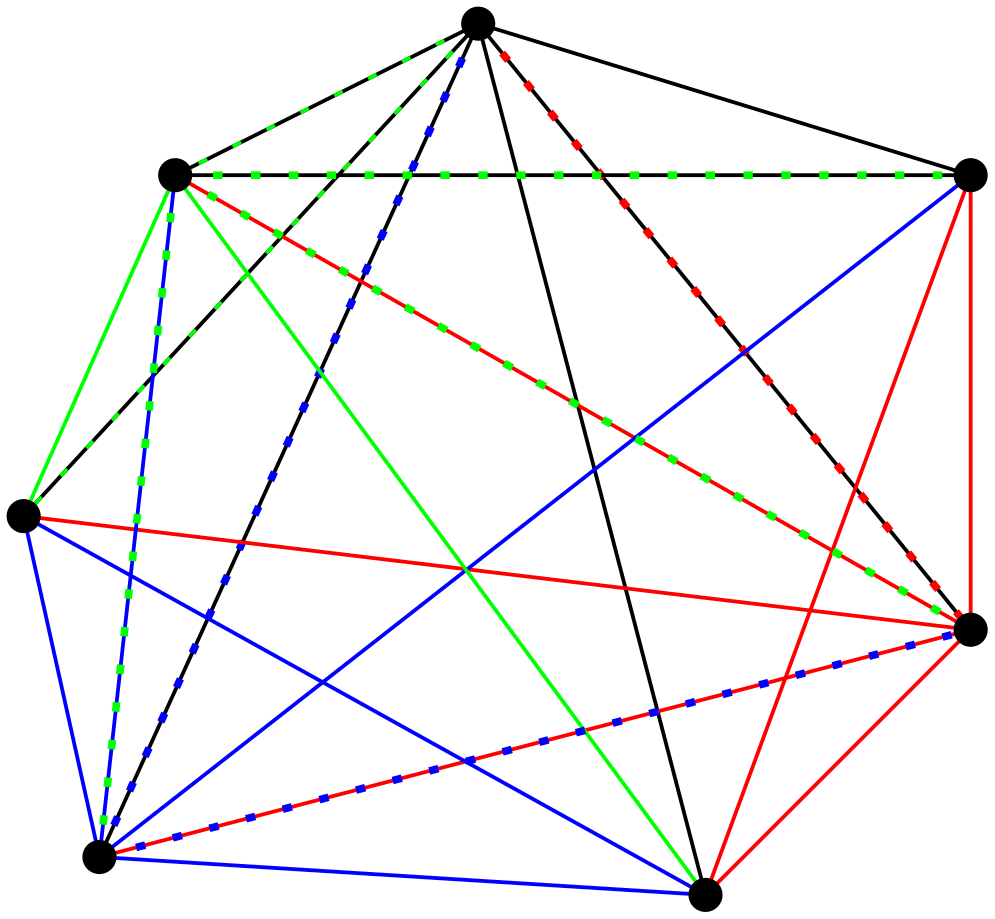
\includegraphics[width=0.75\linewidth]{images/thrackles_maximos}
\end{figure}
\end{frame}

\begin{frame}
\frametitle{Estado del arte : thrackles máximos en posición general}
\pause
\begin{itemize}
	\item En posición general es muy dificil dibujar thrackles máximos que sean disjuntos.
	\item La intuición nos dice que el resultado anterior es válido para posición general.
	\item ¿Cómo probamos \emph{todas} las gráficas geométricas de $K_n$?
\end{itemize}
\end{frame}

\begin{frame}
\frametitle{Tipo de orden}
Aichholzer \emph{et al.} definen el \emph{tipo de orden} de un conjunto $S=\{p_1,p_2,\dots p_n\}$ de puntos en posición general
como una función que asigna a cada tripleta ordenada $i,j,k\in\{1,2,\dots n\}$ la orientación de la tripleta de puntos $\{p_i,p_j,p_k\}$.
\begin{figure}
	\centering
	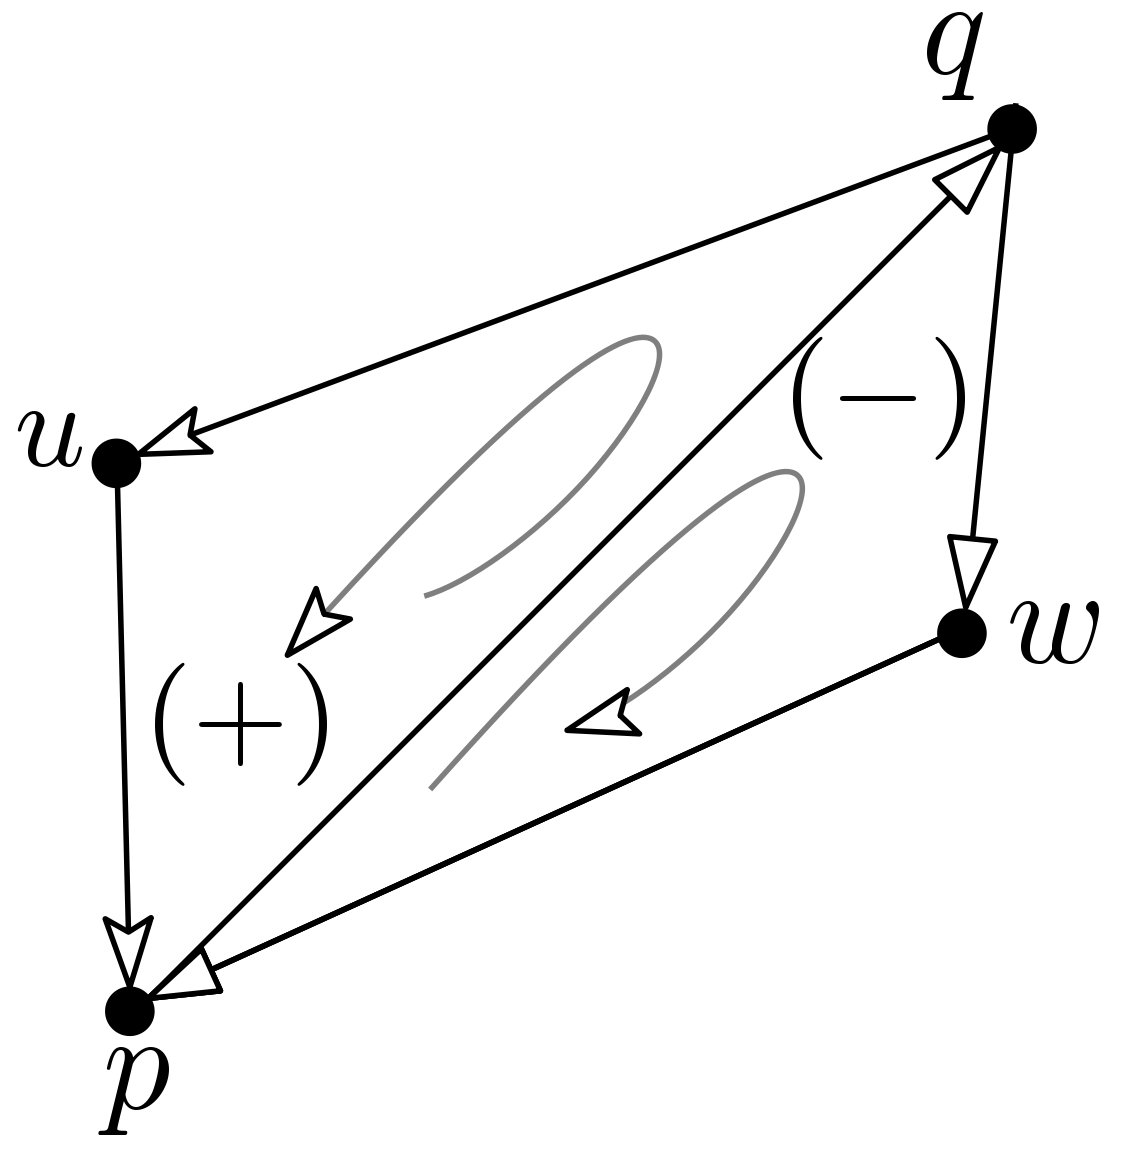
\includegraphics[width=0.3\linewidth]{images/triplet}
\end{figure}
Decimos que dos conjuntos de puntos $S_1$ y $S_2$ son combinatoriamente equivalentes cuando tienen el mismo tipo de orden.
\end{frame}

\begin{frame}
\frametitle{Tipo de orden}
Aichholzer \emph{et al.} ofrecen una base de datos para los tipos de orden de $3 \leq n \leq 10$.
\begin{table}[ht]
	\centering
	\begin{tabular}{|c|c|r|}
		\hline
		$n$ & Número de tipos de orden & Tamaño (bytes)   \\ \hline
		3     & 1                   & 6       \\ \hline
		4     & 2                   & 16      \\ \hline
		5     & 3                   & 30      \\ \hline
		6     & 16                  & 192     \\ \hline
		7     & 135                 & 1890    \\ \hline
		8     & 3315                & 53040   \\ \hline
		9     & 158817              & 5 717 412   \\\hline
		10    & 14309547            & 572 381 880 \\ \hline
	\end{tabular}
	\caption{Tipos de orden para cada $n\leq10$.}
	\label{tab:ots}
\end{table}
\end{frame}
\begin{frame}
\frametitle{Estado del arte : construyendo la nueva cota inferior}
Para analizar cada par de thrackles máximos en algun dibujo de $K_n$, primero hay que encontrarlos. Por ello, construimos un algoritmo 
exhaustivo que usa \emph{backtracking} para encontrar thrackles de cualquier tamaño. Nosotros llamamos $k-$thrackle a un thrackle de tamaño $k$.
Explicar algoritmo de búsqueda de $k$ thrackles y cómo hacemos la intersección.

\end{frame}

\begin{frame}
\frametitle{Estado del arte : construyendo la nueva cota inferior}
Una vez que hicimos las intersecciones de cada par de thrackles máximos en todos los dibujos de $K_n$, con $3 \leq n \leq 10$ encontramos los siguientes resultados:
\begin{itemize}
	\item Para todo tipo de orden con al menos dos thrackles máximos, cada par de thrackles máximos tienen intersección no vacía en aristas.
	\item Existen tipos de orden con solo un thrackle máximo.
	\item Existen tipos de orden en los que no hay thrackles máximos.
\end{itemize}
\end{frame}

\begin{frame}
\frametitle{Estado del arte : construyendo la nueva cota inferior}
Esto nos permite calcular el número exacto de aristas cubiertas, en el mejor caso, por una descomposición que es inducida por una colección de thrackles máximos. 

Nosotros probamos que, $m$ thrackles máximos pueden cubrir a lo sumo:
\[
-\frac{1}{2}m(m-2n-1)
\] aristas de la gráfica completa.
\pause 

\begin{table}
	\centering
\scalebox{0.7}{

	\begin{tabular}{	| >{\centering\arraybackslash}m{0.5in} | >{\centering\arraybackslash}m{0.8in} |  >{\centering\arraybackslash}m{1.2in} |  >{\centering\arraybackslash}m{1in} | }
		\hline
		$n$ & $m = \left\lceil\frac{n-1}{2}\right\rceil$ &     $-\frac{1}{2}m(m-2n-1) $ &
		$\binom{n}{2}$\\[5pt] \hline\hline
		3   & 1  & 3 & 3 \\ \hline
		4   & 2  & 7 & 6 \\ \hline
		5   & 2  & \cellcolor{red!25}9 & 10 \\ \hline
		6   & 3  & 15 & 15 \\ \hline
		7   & 3  & \cellcolor{red!25}18 & 21 \\ \hline
		8   & 4  & \cellcolor{red!25}26 & 28 \\ \hline
		9   & 4  & \cellcolor{red!25}30 & 36 \\ \hline
		10  & 5  & \cellcolor{red!25}40 & 45 \\ \hline
	\end{tabular}
}
\end{table}
\end{frame}

\begin{frame}
\frametitle{Estado del arte : construyendo la nueva cota inferior}
De la misma manera, para saber cuántos thrackles son necesarios para cubrir todas las aristas de la gráfica completa, debemos 
resolver la siguiente desigualdad para $m$:
\[
-\frac{1}{2}m(m-2n-1) \geq \binom{n}{2}.
\]
Usando la ecuación cuadrática encontramos que \[m =  n - \left\lfloor\sqrt{2n + \frac{1}{4}} - \frac{1}{2} \right\rfloor \]

\end{frame}
\begin{frame}
\frametitle{Estado del arte : construyendo la nueva cota inferior}
\begin{table}
	\centering
	\scalebox{0.9}{
		
		\begin{tabular}{	| >{\centering\arraybackslash}m{0.5in} | >{\centering\arraybackslash}m{1.6in} |  >{\centering\arraybackslash}m{1.2in} |  >{\centering\arraybackslash}m{1in} | }
			\hline
			$n$ & $m =  n - \left\lfloor\sqrt{2n + \frac{1}{4}} - \frac{1}{2} \right\rfloor $ &     $-\frac{1}{2}m(m-2n-1) $ &
			$\binom{n}{2}$\\[5pt] \hline\hline
			3   & 1  & 3 & 3 \\ \hline
			4   & 2  & 7 & 6 \\ \hline
			5   & 3  & 12 & 10 \\ \hline
			6   & 3  & 15 & 15 \\ \hline
			7   & 4  & 22 & 21 \\ \hline
			8   & 5  & 30 & 28 \\ \hline
			9   & 6  & 39 & 36 \\ \hline
			10  & 6  & 45 & 45 \\ \hline
		\end{tabular}
	}
\end{table}
Tenemos una nueva cota inferior para $3 \leq n \leq 10$:
\[ At_g(K_n) \geq n - \left\lfloor\sqrt{2n + \frac{1}{4}} - \frac{1}{2} \right\rfloor \] 
\end{frame}
\begin{frame}
\frametitle{Anti-thickness geométrico de $K_n$ para $3\leq n\leq 10$}
Con el resultado anterior y el resultado del estado del arte tenemos que, para $ 3 \leq n \leq 10$:
\[ n - \left\lfloor\sqrt{2n + \frac{1}{4}} - \frac{1}{2} \right\rfloor  \leq At_g(K_n) \leq n - \left\lfloor\sqrt{2n + \frac{1}{4}} - \frac{1}{2} \right\rfloor \] 
\pause
\[ At_g(K_n) = n - \left\lfloor\sqrt{2n + \frac{1}{4}} - \frac{1}{2} \right\rfloor \] 
\end{frame}

\begin{frame}
\frametitle{Anti-thickness geométrico de $K_n$ para $3\leq n\leq 10$}
\begin{itemize}
	\item[] Recordemos que la cota superior fue obtenida encontrando el anti-thickness de un dibujo específico, el que está en posición convexa.
	\item[] Recordemos que si $S$ es un conjunto de $n$ vértices en posición convexa, entonces \[ At_g(K(S)) = \min\{D(S)\} = \max\{D(S)\} = d(n)\]
\end{itemize}
¿Qué pasa con el anti-thickness de dibujos en posición general no convexa?
\end{frame}

\begin{frame}
\frametitle{Anti-thickness de dibujos en posición general no convexa}
\end{frame}
\chapter{Conclusiones y trabajo futuro}
En esta tesis estudiamos el problema del anti-thickness geométrico de gráficas completas con hasta 10
vértices. El anti-thickness geométrico de una gráfica es el entero $k$ más pequeño tal que existe una
descomposición de la gráfica en $k$ thrackles. Un thrackle es una gráfica en la que cada par de aristas se
intersecta exactamente una vez.

En este trabajo encontramos que el anti-thickness geométrico $At_g(K_n)$ de la gráfica completa de $n$
vértices $K_n$, con $ 3 \leq n \leq 10$, es:
\[ At_g(K_n) =  n - \left\lfloor \sqrt{2n + \frac{1}{4}} - \frac{1}{2}\right\rfloor. \]
Para dar este resultado analizamos las gráficas completas inducidas por los conjuntos de hasta diez
vértices proveídos por la base de datos de tipos de orden del trabajo de~\cite{Aichholzer2001}, encontramos
que dos thrackles máximos de la misma gráfica completa comparten al menos una arista, dando así una nueva
cota inferior para conjuntos pequeños de puntos. La cota superior está dada por el anti-thickness del
dibujo de $K_n$ en posición convexa; nosotros encontramos dibujos, que no están en posición convexa, que
tienen el mismo anti-thickness.

Para cada thrackle de las descomposiciones encontradas calculamos el número
de cruce para observar que existe una relación del número de thrackles con número de cruce alto y número de
cruce bajo cercana al 50\%; en este trabajo damos la definición del número de cruce de un thrackle.

También analizamos y listamos cuáles conjuntos de puntos no tienen thrackles máximos y cuáles tienen
solamente un thrackle máximo para cada $n$ en el rango $[3,10]$. Aquí hacemos la observación de que
conjuntos con un número de cruce pequeño tienen menos thrackles máximos que los conjuntos con un número de
cruce elevado con respecto del número de cruce máximo para cada $n$ en el rango anteriormente mencionado.

Para los conjuntos de $n$ puntos, con $3 \leq n \leq 8$ que inducen gráficas completas sin thrackles
máximos analizamos, con un algoritmo exhaustivo, el anti-thickness geométrico de cada uno. Encontramos que
estos dibujos tienen anti-thickness mayor, en una unidad, al anti-thickness geométrico de $K_n$.

Uno de los objetivos de la tesis era obtener el anti-thickness geométrico de $K_n$ con $n\geq 3$. Sin
embargo no fue posible ya que no pudimos probar la generalización del lema~\ref{lema:thdisjuntos} que establece que la intersección entre dos thrackles máximos de un mismo dibujo siempre sucede. Decidimos no invertir más tiempo en la generalización del teorema para dar más resultados acerca de conjuntos pequeño de $n$.

\subsubsection{Trabajo futuro}

La generalización del lema~\ref{lema:thdisjuntos} es el trabajo a futuro más fuerte, de encontrarse, el
problema del anti-thickness geométrico para gráficas completas quedaría resuelto de manera general. Esto
deja abierto el problema de encontrar el anti-thickness de un dibujo en específico de manera eficiente.
Pero, como explicamos en el capítulo~\ref{cap3}, encontrar el anti-thickness de una gráfica geométrica
equivale a encontrar el número cromático de su gráfica de disyunción y este último es un problema
$NP$-difícil~(\cite{Skiena2003}). Sin embargo, existen algoritmos genéticos para encontrar una aproximación
al número cromático de una gráfica dada como los presentados en~\cite{Fleurent1996} y \cite{Galinier1999}
en los que se muestra que los resultados fueron obtenidos en un rango de tiempo considerablemente bueno
para el hardware en el que se implementaron. Es posible implementar estos algoritmos para encontrar la
coloración de la gráfica de disyunción y obtener resultados acerca del anti-thickness de algún dibujo de
$K_n$.

También es deseable encontrar una manera de caracterizar los dibujos que inducen gráficas completas sin
thrackles máximos, o con solo uno, ya que analizar todas las $\displaystyle \binom{\binom{n}{2}}{n}$
posibles combinaciones de $n$ aristas para buscar thrackles máximos puede resultar ineficiente,
especialmente con conjuntos grandes de puntos.

\appendix
\chapter{Etiquetas de thrackles máximos}
\label{apendice_thrackles_inducen}
  \begin{tabular}[t]{|c|c|c|}
    \hline
    $n$                 & Tipo de Orden       & Thrackles             \\ \hline \hline
    \multirow{3}{*}{8}  & \multirow{2}{*}{2}  & 36 32 29 25 2         \\ \cline{3-3}
                        &                     & 37 31 28 23 0         \\ \cline{2-3}
                        & 54                  & 32 29 26 16 2         \\ \hline
    \multirow{23}{*}{9} & 12                  & 101 96 93 68 33 2     \\ \cline{2-3}
                        & 52                  & 100 97 96 92 33 2     \\ \cline{2-3}
                        & 54                  & 82 78 75 52 33 2      \\ \cline{2-3}
                        & \multirow{3}{*}{80} & 71 68 67 55 33 2      \\ \cline{3-3}
                        &                     & 72 68 67 55 33 2      \\ \cline{3-3}
                        &                     & 73 68 59 58 33 2      \\ \cline{3-3}
                        & 696                 & 79 76 73 40 22 2      \\ \cline{2-3}
                        & 1080                & 37 33 32 29 15 2      \\ \cline{2-3}
                        &\multirow{15}{*}{1287}& 57 55 44 35 24 3      \\ \cline{3-3}
                        &                     & 57 56 43 35 24 3      \\ \cline{3-3}
                        &                     & 57 55 50 35 24 3      \\ \cline{3-3}
                        &                     & 57 56 42 35 24 3      \\ \cline{3-3}
                        &                     & 57 56 44 35 24 3      \\ \cline{3-3}
                        &                     & 57 56 45 35 24 3      \\ \cline{3-3}
                        &                     & 57 56 48 35 24 3      \\ \cline{3-3}
                        &                     & 57 56 49 35 24 3      \\ \cline{3-3}
                        &                     & 57 56 50 35 24 3      \\ \cline{3-3}
                        &                     & 57 56 51 35 24 3      \\ \cline{3-3}
                        &                     & 60 56 39 35 24 3      \\ \cline{3-3}
                        &                     & 60 57 56 35 24 3      \\ \cline{3-3}
                        &                     & 61 56 39 35 24 3      \\ \cline{3-3}
                        &                     & 61 57 56 35 24 3      \\ \cline{3-3}
                        &                     & 62 55 39 35 24 3      \\ \hline
  \end{tabular}
  \begin{tabular}[t]{|c|c|c|}
    \hline
    $n$                 &Tipo de Orden        & Thrackles         \\ \hline\hline
    \multirow{25}{*}{9} &\multirow{25}{*}{1287}& 62 56 39 35 24 3      \\ \cline{3-3}
                        &                     & 62 57 55 35 24 3      \\ \cline{3-3}
                        &                     & 62 57 56 35 24 3      \\ \cline{3-3}
                        &                     & 63 56 35 20 6 0      \\ \cline{3-3}
                        &                     & 63 56 35 20 7 6     \\ \cline{3-3}
                        &                     & 63 56 35 21 20 0      \\ \cline{3-3}
                        &                     & 63 56 35 22 20 0      \\ \cline{3-3}
                        &                     & 63 56 35 24 3 0     \\ \cline{3-3}
                        &                     & 63 56 35 24 4 0     \\ \cline{3-3}
                        &                     & 63 56 35 24 5 0     \\ \cline{3-3}
                        &                     & 63 56 35 24 6 0     \\ \cline{3-3}
                        &                     & 63 56 35 24 7 3     \\ \cline{3-3}
                        &                     & 63 56 35 24 7 4     \\ \cline{3-3}
                        &                     & 63 56 35 24 7 5     \\ \cline{3-3}
                        &                     & 63 56 35 24 7 6     \\ \cline{3-3}
                        &                     & 63 56 35 24 12 0      \\ \cline{3-3}
                        &                     & 63 56 35 24 13 0      \\ \cline{3-3}
                        &                     & 63 56 35 24 14 0      \\ \cline{3-3}
                        &                     & 63 56 35 24 15 0      \\ \cline{3-3}
                        &                     & 63 56 35 24 17 0      \\ \cline{3-3}
                        &                     & 63 56 35 24 18 0      \\ \cline{3-3}
                        &                     & 63 56 35 24 21 0      \\ \cline{3-3}
                        &                     & 63 56 35 24 22 0      \\ \cline{3-3}
                        &                     & 63 56 39 35 24 3      \\ \cline{3-3}
                        &                     & 63 57 56 35 24 3      \\ \hline

  \end{tabular}
  \begin{tabular}[p]{|c|c|c|}
    \hline
    $n$                 &Tipo de Orden        & Thrackles         \\ \hline\hline
    \multirow{4}{*}{10} & 81                  & 176 168 156 125 38 0 \\ \cline{2-3}
                        & 1328                &150 142 113 100 39 0 \\ \cline{2-3}
                        & \multirow{2}{*}{2243}& 121 119 85 67 42 3 \\ \cline{3-3}
                        &                     & 128 115 82 51 39 0 \\ \hline
  \end{tabular}

\chapter{Números de cruce para thrackles máximos}
\label{apendice_thrackles_inducen_cn}
  \begin{tabular}[t]{|c|c|c|c|}
    \hline
    $n$                 & Tipo de Orden       & Thrackles             & Números de Cruce\\ \hline \hline
    \multirow{3}{*}{8}  & \multirow{2}{*}{12} & 36 32 29 25 2         & 5 5 11 5 11     \\ \cline{4-4}
                        &                     & 37 31 28 23 0         & 11 5 5 11 5     \\ \cline{2-4}
                        & 54                  & 32 29 26 16 2         & 5 5 11 5 11     \\ \hline
    \multirow{23}{*}{9} & 12                  & 101 96 93 68 33 2     & 14 6 14 14 6 6  \\ \cline{2-4}
                        & 52                  & 100 97 96 92 33 2     & 14 6 14 6 6 6   \\ \cline{2-4}
                        & 54                  & 82 78 75 52 33 2      & 6 6 14 14 6 14  \\ \cline{2-4}
                        & \multirow{3}{*}{80} & 71 68 67 55 33 2      & 14 6 15 6 6 14  \\ \cline{4-4}
                        &                     & 72 68 67 55 33 2      & 14 6 15 6 6 11  \\ \cline{4-4}
                        &                     & 73 68 59 58 33 2      & 6 6 17 6 6 14   \\ \cline{4-4}
                        & 696                 & 79 76 73 40 22 2      & 14 6 14 14 6 6  \\ \cline{2-4}
                        & 1080                & 37 33 32 29 15 2      & 14 6 14 18 6 6  \\ \cline{2-4}
                        &\multirow{15}{*}{1287}& 57 55 44 35 24 3     & 6 11 11 15 6 15 \\ \cline{4-4}
                        &                     & 57 56 43 35 24 3      & 6 11 14 15 6 15 \\ \cline{4-4}
                        &                     & 57 55 50 35 24 3      & 6 6 20 15 6 15  \\ \cline{4-4}
                        &                     & 57 56 42 35 24 3      & 6 6 17 15 6 15  \\ \cline{4-4}
                        &                     & 57 56 44 35 24 3      & 6 6 11 15 6 15  \\ \cline{4-4}
                        &                     & 57 56 45 35 24 3      & 6 6 21 15 6 15  \\ \cline{4-4}
                        &                     & 57 56 48 35 24 3      & 6 6 22 15 6 15  \\ \cline{4-4}
                        &                     & 57 56 49 35 24 3      & 6 6 20 15 6 15  \\ \cline{4-4}
                        &                     & 57 56 50 35 24 3      & 6 6 14 15 6 15  \\ \cline{4-4}
                        &                     & 57 56 51 35 24 3      & 6 6 22 15 6 15  \\ \cline{4-4}
                        &                     & 60 56 39 35 24 3      & 14 6 11 15 6 15 \\ \cline{4-4}
                        &                     & 60 57 56 35 24 3      & 14 6 11 15 6 15 \\ \cline{4-4}
                        &                     & 61 56 39 35 24 3      & 14 6 6 15 6 15  \\ \cline{4-4}
                        &                     & 61 57 56 35 24 3      & 11 6 11 15 6 15 \\ \cline{4-4}
                        &                     & 62 55 39 35 24 3      & 11 6 6 15 6 15  \\ \hline
  \end{tabular}
\\
  \begin{tabular}[t]{|c|c|c|c|}

    \hline
    $n$                 &Tipo de Orden        & Thrackles          & Número de cruce  \\ \hline\hline
    \multirow{25}{*}{9} &\multirow{25}{*}{1287}& 62 56 39 35 24 3  & 6 6 11 15 6 15   \\ \cline{3-3}
                        &                     & 62 57 55 35 24 3   & 6 6 11 15 6 15  \\ \cline{3-3}
                        &                     & 62 57 56 35 24 3   & 6 6 6 15 6 15  \\ \cline{3-3}
                        &                     & 63 56 35 20 6 0    & 15 6 15 11 6 6 \\ \cline{3-3}
                        &                     & 63 56 35 20 7 6    & 15 6 15 11 11 6 \\ \cline{3-3}
                        &                     & 63 56 35 21 20 0   & 15 6 15 11 11 6  \\ \cline{3-3}
                        &                     & 63 56 35 22 20 0   & 15 6 15 14 11 6  \\ \cline{3-3}
                        &                     & 63 56 35 24 3 0    & 15 6 15 6 15 6 \\ \cline{3-3}
                        &                     & 63 56 35 24 4 0    & 15 6 15 6 14 6 \\ \cline{3-3}
                        &                     & 63 56 35 24 5 0    & 15 6 15 6 11 6 \\ \cline{3-3}
                        &                     & 63 56 35 24 6 0    & 15 6 15 6 6 6 \\ \cline{3-3}
                        &                     & 63 56 35 24 7 3    & 15 6 15 6 11 15 \\ \cline{3-3}
                        &                     & 63 56 35 24 7 4    & 15 6 15 6 11 14 \\ \cline{3-3}
                        &                     & 63 56 35 24 7 5    & 15 6 15 6 11 11 \\ \cline{3-3}
                        &                     & 63 56 35 24 7 6    & 15 6 15 6 11 6 \\ \cline{3-3}
                        &                     & 63 56 35 24 12 0   & 15 6 15 6 21 6  \\ \cline{3-3}
                        &                     & 63 56 35 24 13 0   & 15 6 15 6 22 6  \\ \cline{3-3}
                        &                     & 63 56 35 24 14 0   & 15 6 15 6 20 6  \\ \cline{3-3}
                        &                     & 63 56 35 24 15 0   & 15 6 15 6 22 6  \\ \cline{3-3}
                        &                     & 63 56 35 24 17 0   & 15 6 15 6 17 6  \\ \cline{3-3}
                        &                     & 63 56 35 24 18 0   & 15 6 15 6 20 6  \\ \cline{3-3}
                        &                     & 63 56 35 24 21 0   & 15 6 15 6 11 6  \\ \cline{3-3}
                        &                     & 63 56 35 24 22 0   & 15 6 15 6 14 6  \\ \cline{3-3}
                        &                     & 63 56 39 35 24 3   & 15 6 11 15 6 15  \\ \cline{3-3}
                        &                     & 63 57 56 35 24 3   & 15 6 6 15 6 15  \\ \hline

  \end{tabular}
  \\
  \begin{tabular}[p]{|c|c|c|c|}
    \hline
    $n$                 &Tipo de Orden        & Thrackles            &Número de cruce \\ \hline\hline
    \multirow{4}{*}{10} & 81                  & 176 168 156 125 38 0 & 19 7 19 7 19 7 \\ \cline{2-3}
                        & 1328                &150 142 113 100 39 0  & 19 7 19 7 19 7 \\ \cline{2-3}
                        & \multirow{2}{*}{2243}& 121 119 85 67 42 3  & 7 19 7 19 7 19  \\ \cline{3-3}
                        &                     & 128 115 82 51 39 0   & 19 7 19 7 19 7 \\ \hline
  \end{tabular}

\chapter{Tipos de orden con descomposiciones.}
Presentamos los doce tipos de orden para los cuales existe una descomposición en thrackles máximos.
\begin{figure}[h]
    \centering
    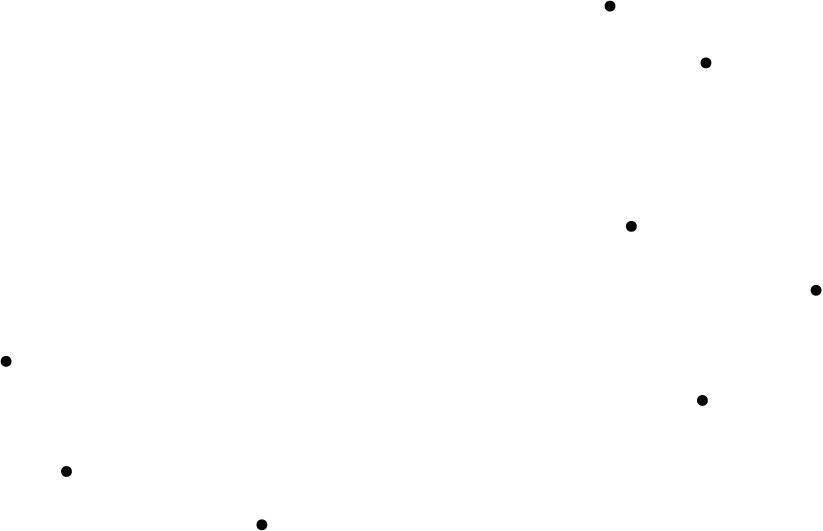
\includegraphics[width=0.8\linewidth, frame]{8_12.png}
    \caption{Tipo de orden número 12 para $n=8$}
\end{figure}
\begin{figure}
    \centering
    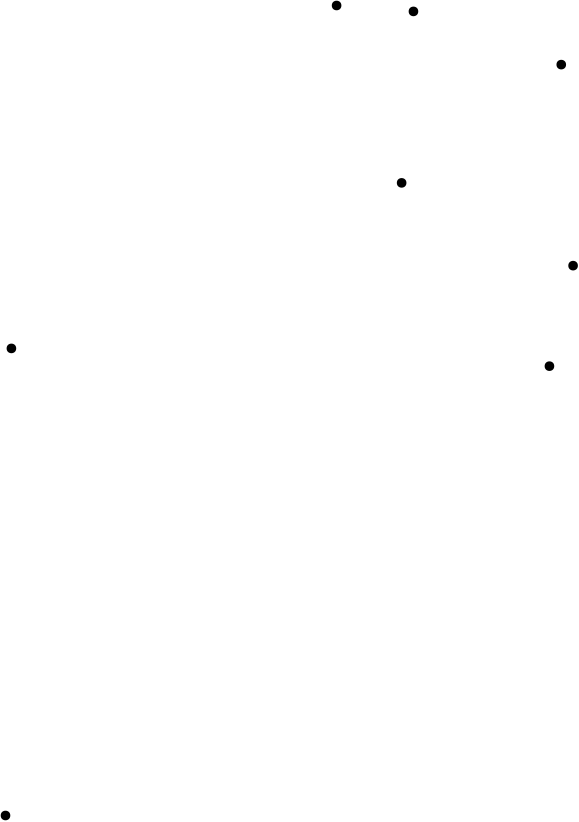
\includegraphics[width=0.8\linewidth, frame]{8_54.png}
    \caption{Tipo de orden número 54 para $n=8$}
\end{figure}
\begin{figure}
    \centering
    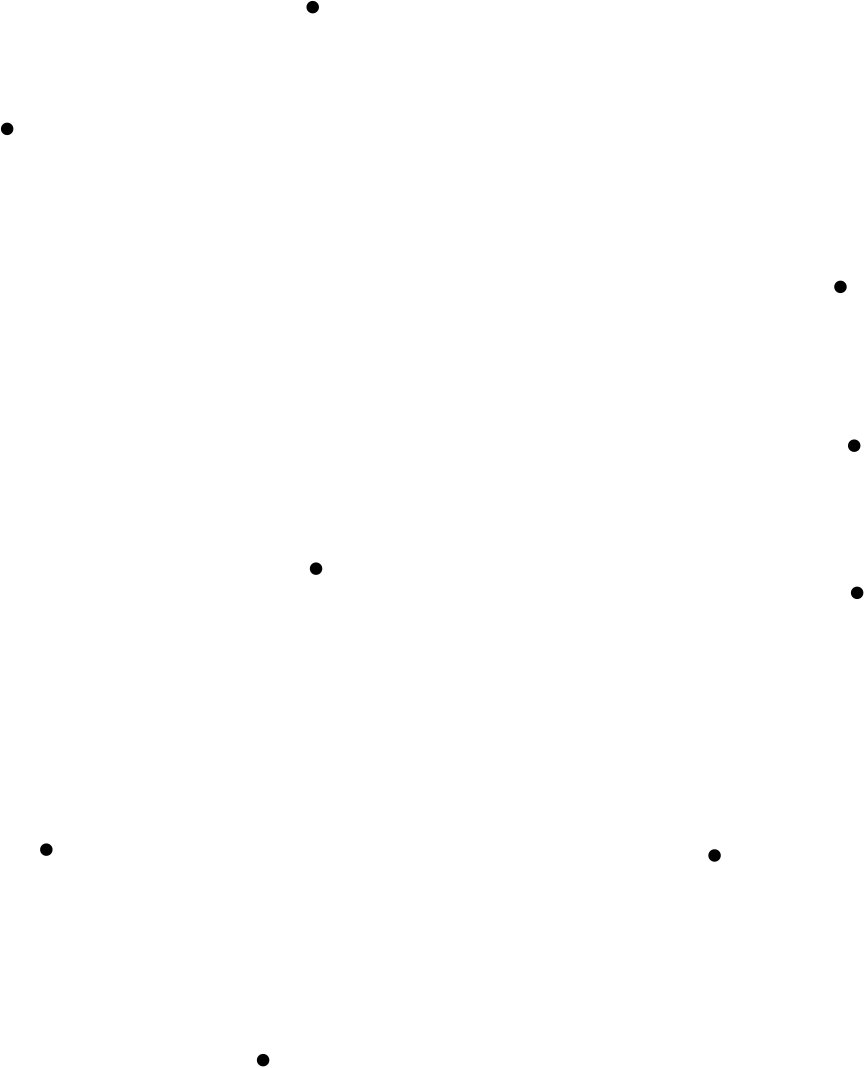
\includegraphics[width=0.8\linewidth, frame]{9_12.png}
    \caption{Tipo de orden número 12 para $n=9$}
\end{figure}
\begin{figure}
    \centering
    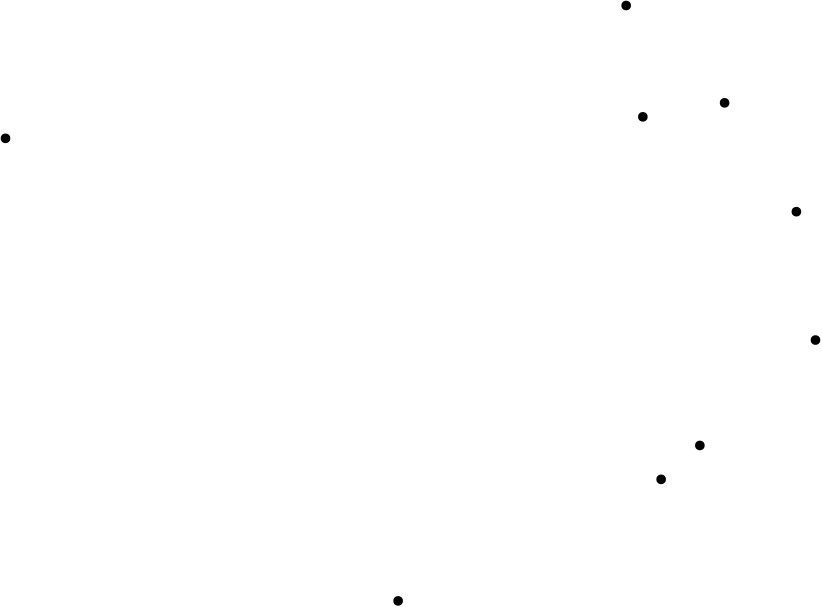
\includegraphics[width=0.9\linewidth, frame]{9_52.png}
    \caption{Tipo de orden número 52 para $n=9$}
\end{figure}
\begin{figure}
    \centering
    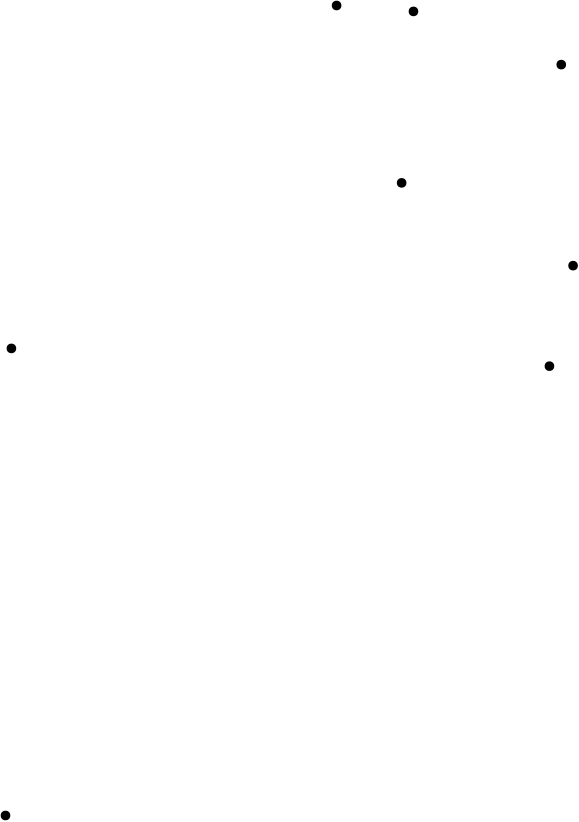
\includegraphics[width=0.9\linewidth, frame]{9_54.png}
    \caption{Tipo de orden número 54 para $n=9$}
\end{figure}
\begin{figure}
    \centering
    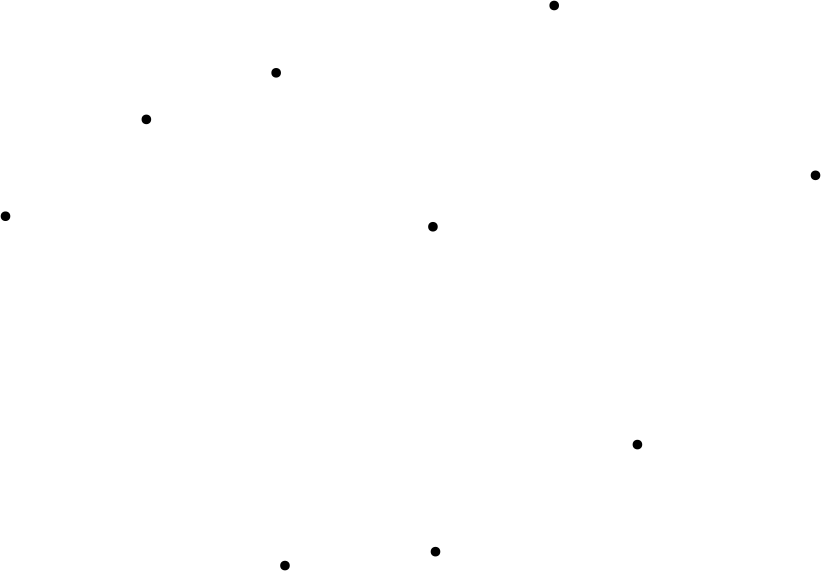
\includegraphics[width=0.9\linewidth, frame]{9_80.png}
    \caption{Tipo de orden número 80 para $n=9$}
\end{figure}
\begin{figure}
    \centering
    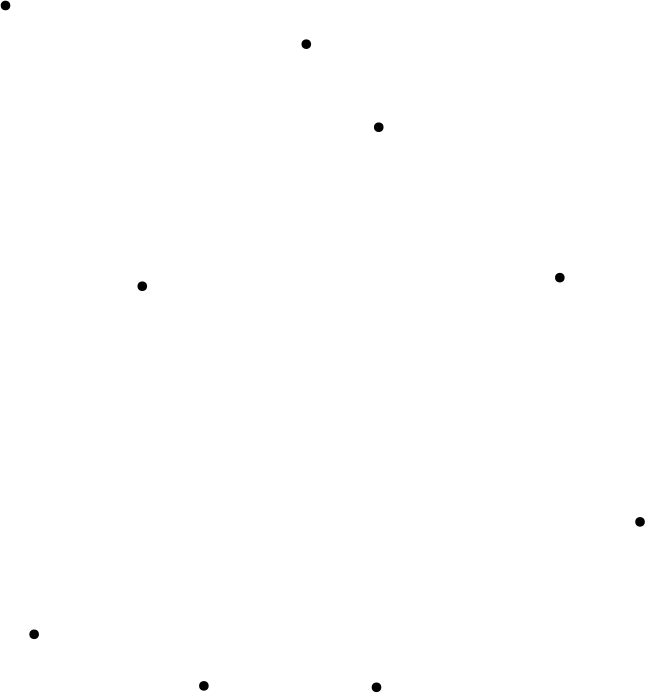
\includegraphics[width=0.9\linewidth, frame]{9_696.png}
    \caption{Tipo de orden número 696 para $n=9$}
\end{figure}

\begin{figure}
    \centering
    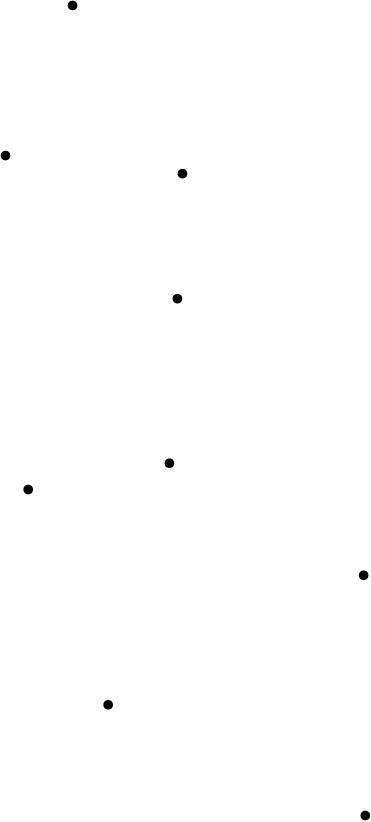
\includegraphics[width=0.6\linewidth, frame]{9_1080.png}
    \caption{Tipo de orden número 1080 para $n=9$}
\end{figure}
\begin{figure}
    \centering
    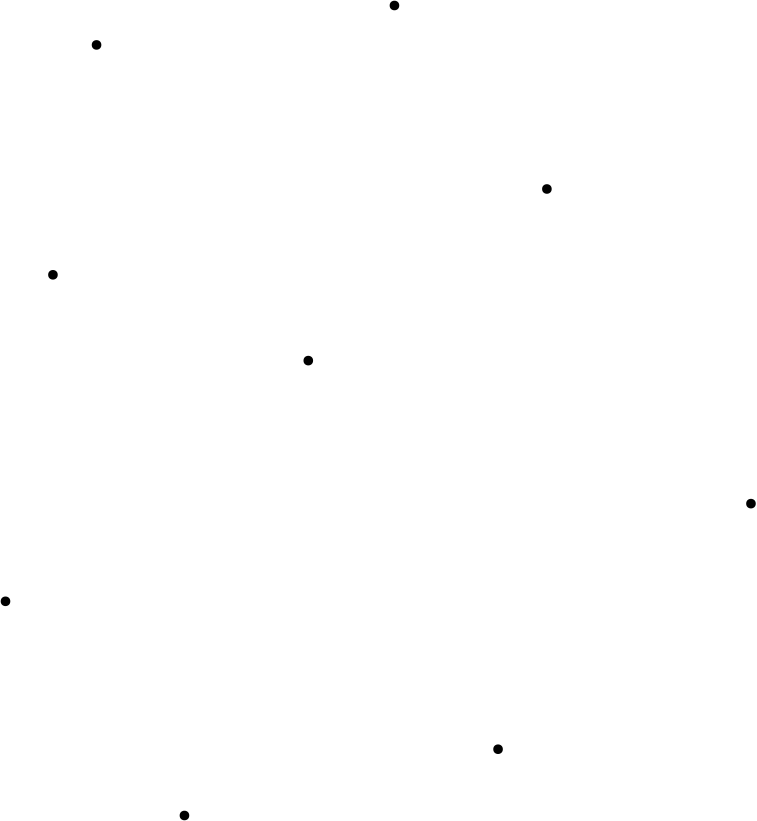
\includegraphics[width=0.9\linewidth, frame]{9_1287.png}
    \caption{Tipo de orden número 1287 para $n=9$}
\end{figure}
\begin{figure}
    \centering
    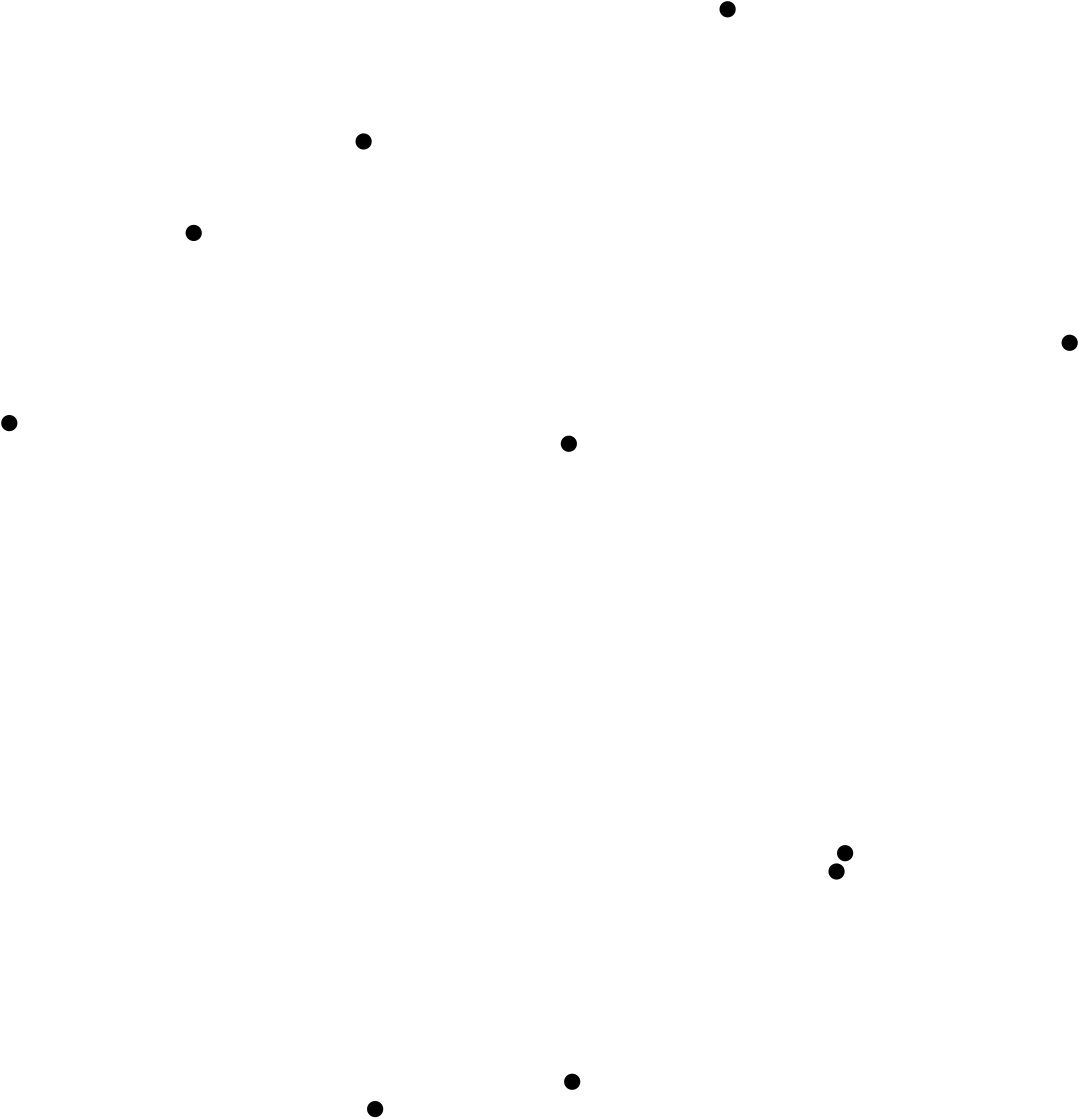
\includegraphics[width=\linewidth, frame]{10_81.png}
    \caption{Tipo de orden número 81 para $n=10$}
\end{figure}
\begin{figure}
    \centering
    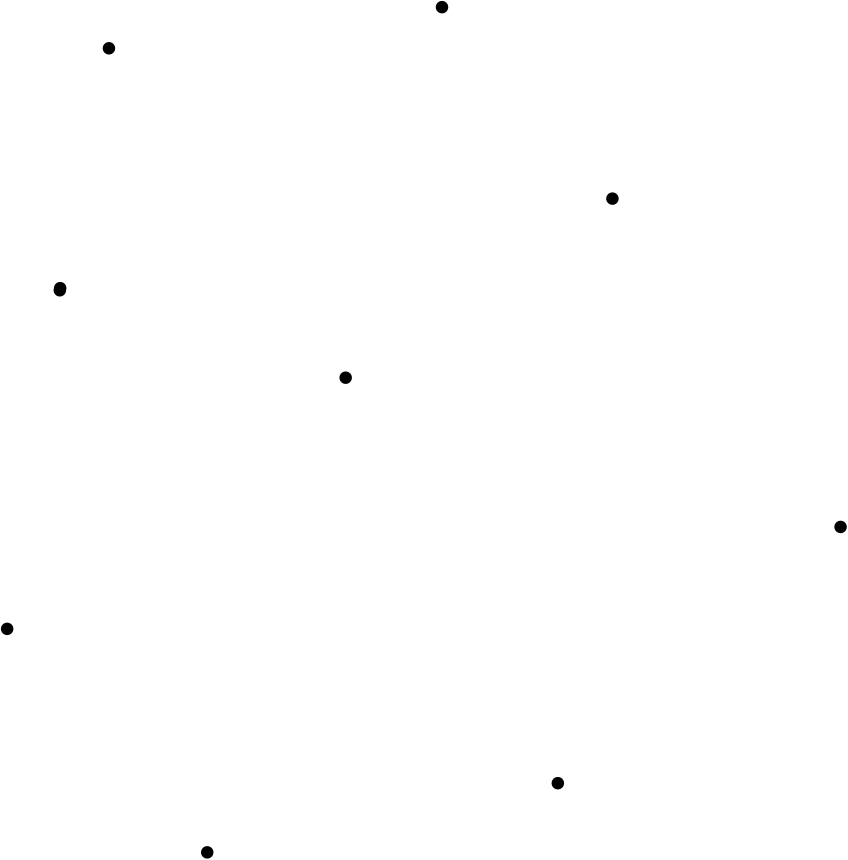
\includegraphics[width=\linewidth, frame]{10_1328.png}
    \caption{Tipo de orden número 1328 para $n=10$}
\end{figure}
\begin{figure}
    \centering
    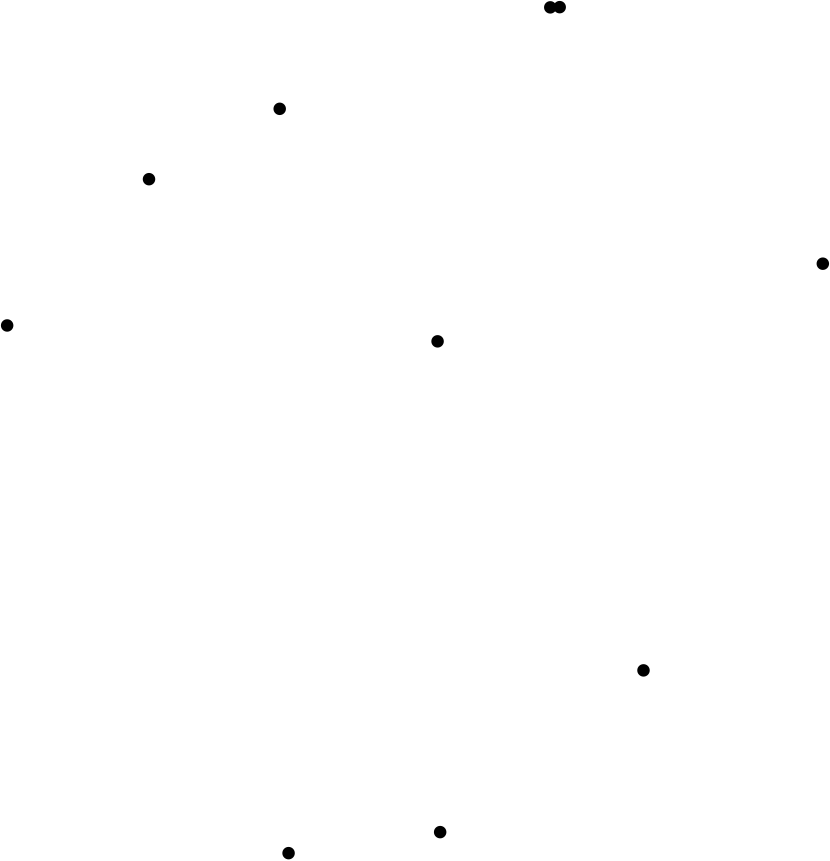
\includegraphics[width=\linewidth, frame]{10_2243.png}
    \caption{Tipo de orden número 2243 para $n=10$}
\end{figure}

\chapter{Lista de ligas.}
\label{apendice-ligas}
\begin{enumerate}
  \item Tipos de orden con solo un thrackle máximo.
  \label{link-withone}
  \url{http://computacion.cs.cinvestav.mx/~dmerinos/site/archivos_tesis/withone_max.tar.gz}.
  \item Thrackles máximos por cada tipo de orden ordenados por número de thrackles máximos.
  \label{link-thrMax_k}
  \url{http://computacion.cs.cinvestav.mx/~dmerinos/site/archivos_tesis/thrMax_k.tar.xz}
  \item Thrackles máximos para cada tipo de orden de 3 a 9 puntos.
  \label{link-3to9}
  \url{http://computacion.cs.cinvestav.mx/~dmerinos/site/archivos_tesis/3to9.tar.gz}
  \item Thrackles máximos para cada tipo de orden de 10 puntos.
  \label{link-10}
  \url{http://computacion.cs.cinvestav.mx/~dmerinos/site/archivos_tesis/10.tar.gz}
  \item Tipos de orden que no tienen thrackles máximos.
  \label{link-thrWithoutMax}
  \url{http://computacion.cs.cinvestav.mx/~dmerinos/site/archivos_tesis/without_max.tar.gz}
  \item Anti-thickness de los dibujos para los cuales no hay thrackles máximos.
  \label{link-thrWithoutMax-at}
  \url{http://computacion.cs.cinvestav.mx/~dmerinos/site/archivos_tesis/without_max_at.tar.gz}
  \item Funciones programadas en este proyecto
  \label{link-github}
  \url{https://github.com/demaseme/programas_tesis_rev3/tree/master/cpps}.
\end{enumerate}

\bibliographystyle{apa-good.bst}
\bibliography{bibliografia.bib}
\end{document}
